%% abtex2-modelo-artigo.tex, v-1.9.7 laurocesar
%% Copyright 2012-2018 by abnTeX2 group at http://www.abntex.net.br/ 
%%
%% This work may be distributed and/or modified under the
%% conditions of the LaTeX Project Public License, either version 1.3
%% of this license or (at your option) any later version.
%% The latest version of this license is in
%%   http://www.latex-project.org/lppl.txt
%% and version 1.3 or later is part of all distributions of LaTeX
%% version 2005/12/01 or later.
%%
%% This work has the LPPL maintenance status `maintained'.
%% 
%% The Current Maintainer of this work is the abnTeX2 team, led
%% by Lauro César Araujo. Further information are available on 
%% http://www.abntex.net.br/
%%
%% This work consists of the files abntex2-modelo-artigo.tex and
%% abntex2-modelo-references.bib
%%

% ------------------------------------------------------------------------
% ------------------------------------------------------------------------
% abnTeX2: Modelo de Artigo Acadêmico em conformidade com
% ABNT NBR 6022:2018: Informação e documentação - Artigo em publicação 
% periódica científica - Apresentação
% ------------------------------------------------------------------------
% ------------------------------------------------------------------------

\documentclass[
	% -- opções da classe memoir --
	article,			% indica que é um artigo acadêmico
	11pt,				% tamanho da fonte
	oneside,			% para impressão apenas no recto. Oposto a twoside
	a4paper,			% tamanho do papel. 
	% -- opções da classe abntex2 --
	%chapter=TITLE,		% títulos de capítulos convertidos em letras maiúsculas
	%section=TITLE,		% títulos de seções convertidos em letras maiúsculas
	%subsection=TITLE,	% títulos de subseções convertidos em letras maiúsculas
	%subsubsection=TITLE % títulos de subsubseções convertidos em letras maiúsculas
	% -- opções do pacote babel --
	english,			% idioma adicional para hifenização
	brazil,				% o último idioma é o principal do documento
	sumario=tradicional
	]{abntex2}


% ---
% PACOTES
% ---

% ---
% Pacotes fundamentais 
% ---
\usepackage{lmodern}			% Usa a fonte Latin Modern
\usepackage[T1]{fontenc}		% Selecao de codigos de fonte.
\usepackage[utf8]{inputenc}		% Codificacao do documento (conversão automática dos acentos)
\usepackage{indentfirst}		% Indenta o primeiro parágrafo de cada seção.
\usepackage{nomencl} 			% Lista de simbolos
\usepackage{color}				% Controle das cores
\usepackage{graphicx}			% Inclusão de gráficos
\usepackage{microtype} 			% para melhorias de justificação
\usepackage[]{algorithm2e}
% ---
		
% ---
% Pacotes adicionais, usados apenas no âmbito do Modelo Canônico do abnteX2
% ---
\usepackage{lipsum}				% para geração de dummy text
% ---
		
% ---
% Pacotes de citações
% ---
\usepackage[brazilian,hyperpageref]{backref}	 % Paginas com as citações na bibl
\usepackage[alf]{abntex2cite}	% Citações padrão ABNT
% ---

% ---
% Configurações do pacote backref
% Usado sem a opção hyperpageref de backref
\renewcommand{\backrefpagesname}{Citado na(s) página(s):~}
% Texto padrão antes do número das páginas
\renewcommand{\backref}{}
% Define os textos da citação
\renewcommand*{\backrefalt}[4]{
	\ifcase #1 %
		Nenhuma citação no texto.%
	\or
		Citado na página #2.%
	\else
		Citado #1 vezes nas páginas #2.%
	\fi}%
% ---

% --- Informações de dados para CAPA e FOLHA DE ROSTO ---
\titulo{Proposta de solução do Problema de Dominação de Rainhas Utilizando ILS}
\tituloestrangeiro{Proposed solution to the Minimum Dominating Set of Queens Problem using ILS}


\autor{Maria Edoarda Vallim Fonseca \and Thales Athayde Santos}
%\email{medoarda@id.uff.br}
%\email{thalesathaydesantos@id.uff.br}

\local{Brasil}
\data{2018, v-1.0.0}
% ---

% ---
% Configurações de aparência do PDF final

% alterando o aspecto da cor azul
\definecolor{blue}{RGB}{41,5,195}

% informações do PDF
\makeatletter
\hypersetup{
     	%pagebackref=true,
		pdftitle={\@title}, 
		pdfauthor={\@author},
    	pdfsubject={Proposta de solução do Problema de Dominação de Rainhas Utilizando ILS},
	    pdfcreator={LaTeX with abnTeX2},
		pdfkeywords={ILS}{Algoritmo Genético}{Problema de Dominação de Rainhas}, 
		colorlinks=true,       		% false: boxed links; true: colored links
    	linkcolor=blue,          	% color of internal links
    	citecolor=blue,        		% color of links to bibliography
    	filecolor=magenta,      		% color of file links
		urlcolor=blue,
		bookmarksdepth=4
}
\makeatother
% --- 

% ---
% compila o indice
% ---
\makeindex
% ---

% ---
% Altera as margens padrões
% ---
\setlrmarginsandblock{3cm}{3cm}{*}
\setulmarginsandblock{3cm}{3cm}{*}
\checkandfixthelayout
% ---

% --- 
% Espaçamentos entre linhas e parágrafos 
% --- 

% O tamanho do parágrafo é dado por:
\setlength{\parindent}{1.3cm}

% Controle do espaçamento entre um parágrafo e outro:
\setlength{\parskip}{0.2cm}  % tente também \onelineskip

% Espaçamento simples
\SingleSpacing


% ----
% Início do documento
% ----
\begin{document}

% Seleciona o idioma do documento (conforme pacotes do babel)
%\selectlanguage{english}
\selectlanguage{brazil}

% Retira espaço extra obsoleto entre as frases.
\frenchspacing 

% ----------------------------------------------------------
% ELEMENTOS PRÉ-TEXTUAIS
% ----------------------------------------------------------

%---
%
% Se desejar escrever o artigo em duas colunas, descomente a linha abaixo
% e a linha com o texto ``FIM DE ARTIGO EM DUAS COLUNAS''.
% \twocolumn[    		% INICIO DE ARTIGO EM DUAS COLUNAS
%
%---

% página de titulo principal (obrigatório)
\maketitle


% titulo em outro idioma (opcional)



% resumo em português
\begin{figure}
centering
  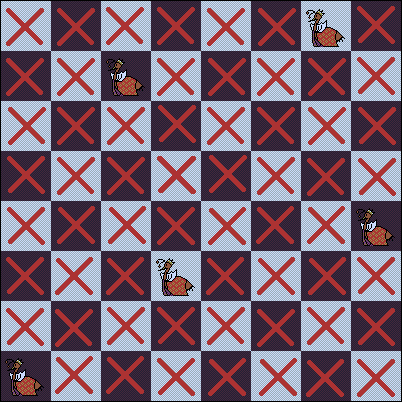
\includegraphics[width=0.60\linewidth]{dom2rainha8x8.png}
  \caption{Exemplo de um tabuleiro de tamanho \textit{8x8} sendo completamente dominado por
  quatro rainhas}
  \label{fig:2rainha}
\end{figure}

Figure \ref{fig:2rainha} shows a sdfsdfwererWboat.

Um problema semelhante, proposto em 1850, conhecido como problema das n-rainhas teve muitos esforços focados nele para sua solução. O problema das n-rainhas é descrito como: dado um tabuleiro nxn, qual seria a disposição das rainhas de modo que nenhuma rainha consiga atacar a outra. Houve muita pesquisa em torno deste problema, e suas soluções utilizam desde teoria matemática até teoria dos grafos. O estudo desse tipo de problema pode beneficiar várias áreas como controle de tráfego, prevenção de \textit{deadlocks} e armazenamento de memória paralela.~\cite{bell2009survey}


%%%%%%%%%%%%%%%%%%%%%%%%%%%%%%%%%%%%%%%%%%%%%%%%%%%%%%%%%%%%%%%%%%%%%%

\section{Methodology}

O \textit{Local Search} foi implementado com 1 de distância pela nossa implementação estar utilizando uma matriz e não um vetor contendo todas as posições do tabuleiro. Embora usar um \textit{Local Search} com distâncias maiores gere resultados melhores, isso teria a consequência negativa de aumentar exponencialmente o tempo computacional da execução do algoritmo.

Pseudocódigo do ILS
\begin{algorithm}
  \KwData{rainhas, best, maxIterações}
  \KwResult{best - melhor solução }
  $rainhas \gets randomStart(rainhas)$\;
  $rainhas \gets Local Search(rainhas)$\;
  $best \gets rainhas$\;
  \Repeat{$max Iterações$ OU $fitness(best)=1$}{
   $rainhas \gets perturbation(rainhas)$\;
   $rainhas \gets Local Search(rainhas)$\;
   \If{$fitness(rainhas)>fitness(best)$}{
     $best \gets rainhas$\;
   }
  }
  \caption{Pseudocódigo do algoritmo de ILS utilizado}
 \end{algorithm}

 \begin{algorithm}
  \KwData{rainhas, tabuleiro}
  \KwResult{how to write algorithm with \LaTeX2e }
  initialization\;
  listaMovimentos = [0..7]\;
  melhorResultado\;
  \While{rainhas}{
  
   embaralha(rainhas)\;
   \eIf{understand}{
    go to next section\;
    current section becomes this one\;
    }{
    go back to the beginning of current section\;
   }
  }
  \caption{Pseudocódigo do Algoritmo Genético utilizado}
 \end{algorithm}
 

%%%%%%%%%%%%%%%%%%%%%%%%%%%%%%%%%%%%%%%%%%%%%%%%%%%%%%%%%%%%%%%%%%%%%%
\section{Resultados}

Nossos testes foram rodados em uma máquina Intel Core i5-7200U com 8GB de RAM, usando o sistema operacional Manjaro Linux com o pacote gráfico KDE Plasma. A linguagem de programação utilizada foi Python 3.7.1.

%%%%%%%%%%%%%%%%%%%%%%%%%%%%%%%%%%%%%%%%%%%%%%%%%%%%%%%%%%%%%%%%%%%%%%
\section{Conclusão}

Text...
\bookmarksetup{startatroot}% 
% ---

% ----------------------------------------------------------
% ELEMENTOS PÓS-TEXTUAIS
% ----------------------------------------------------------
\postextual

% ----------------------------------------------------------
% Referências bibliográficas
% ----------------------------------------------------------
%\bibliography{abnt}
\bibliography{bibliography}

\end{document}
